\section{Referencial teórico}

Este projeto de pesquisa tem como base de estudo três grandes áreas: sistemas de diagnóstico assistido por computador, redes neurais convolucionais e processamento digital de imagens. De forma individual, cada uma dessas áreas pode ter aplicações em diferentes setores, porém, com os avanços e a popularidade do uso de técnicas de \gls{ia} na saúde, a relação entre essas áreas de estudo está cada vez mais forte. Essa seção está divida entre as áreas de estudo e aplicação do projeto, sendo inteligência artificial e sistemas CAD respectivamente.


\subsection{Sobre Redes Neurais Artificiais}

Segundo Russell e Norvig (2010), a Inteligência Artificial  é um campo da computação que estuda a construção de entidades inteligentes, ou seja, máquinas que parecem ter inteligência humana. A construção dessas entidades se beneficiou de diversas áreas de estudo, como por exemplo: filosofia, matemática, economia, neurociência, psicologia, engenharia da computação, linguística, teoria do controle, cibernética e linguística.


Dentro do campo de estudo da inteligência artificial, uma subárea muito importante é o aprendizado de máquina. Aprendizado de máquina envolve o estudo e aplicação de algoritmos que possam aprender a partir de dados, esses algoritmos aprimoram seu desempenho em uma tarefa à medida que são expostos a mais dados. Dentro dessa área de estudo existem três tipos de aprendizados, aprendizado não supervisionado, em que durante o aprendizado o agente aprende padrões de uma entrada mesmo sem ter recebido valores de saída explícitos; aprendizado por reforço, no qual o sistema aprende a partir de uma série de reforços, que são sinais para as decisões do agente, sejam negativos caso a decisão seja ruim, ou positivo em uma boa decisão; e por último, um tipo de aprendizado muito popular para o treinamento de sistemas \gls{cad}, o aprendizado supervisionado, nesse tipo de aprendizado, o sistema recebe um conjunto de dados e suas respostas, e ao decorrer das iterações o modelo aprende a função que mapeia a entrada com a saída \cite{haykin2009neural}.

As técnicas de aprendizado de máquina tiveram grande impacto neste estudo, possibilitando o treinamento do sistema proposto. Mais especificamente, foi implementado aprendizado profundo (\textit{Deep learning} (DL)), esse campo concentra uma ampla família de técnicas de aprendizado de máquina em que as hipóteses assumem a forma de circuitos algébricos complexos com forças de conexão ajustáveis. O termo ‘profundo’ refere-se ao fato de que esses sistemas geralmente estão organizados em camadas \cite{10.5555/1671238}.

Os sistemas baseados em redes neurais surgiram a partir do desafio de resolver problemas complexos que são inviáveis de solucionar com paradigmas tradicionais de programação. Esses sistemas são inspirados no funcionamento do neurônio humano, nesse caso um neurônio artificial, também conhecido como \textit{perceptron}.

\begin{figure}[h]
\centering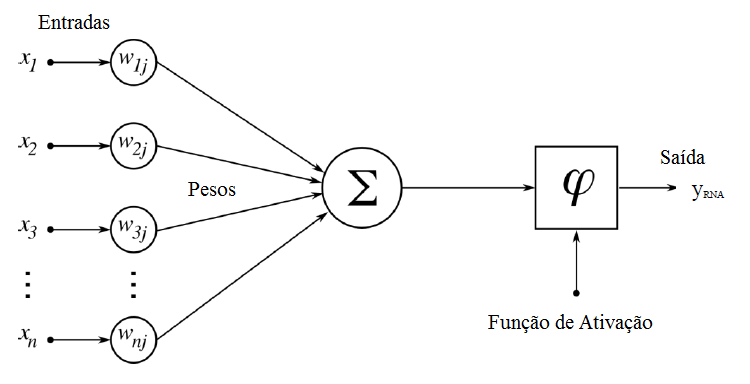
\includegraphics[scale=0.4]{images/Figura-1-neuronio-artificial.png}
\caption{Exemplo do modelo perceptron \cite{imagemperceptron}.}
\label{fig: perceptron}
\end{figure}

O modelo do perceptron, demonstrado na figura \ref{fig: perceptron}, é composto por algumas características principais: Um número $n$ de entradas, em que cada entrada será ponderada por seu respectivo peso $w$, e um termo de viés \(b\) (\textot{bias}). O funcionamento desse neurônio se inicia com uma combinação linear, que é a soma ponderada das entradas $x$ e dos pesos $w$, essa operação pode ser representada como: \(z = w_1  x_1 + ... + w_n  x_n\)  . O resultado dessa operação $(z)$ é passado então a uma função de ativação . Essa função de ativação tem a capacidade de amplificar o aprendizado desses sistemas, já que é essa função que determina se o neurônio será ativado ou não. Essa função de ativação é responsável por aplicar uma transformação não linear à saída da primeira operação, resultando na operação final representada por \(  \sigma  = f(z + b)\) , em que $b$ é termo de viés e $z$ o resultado do somatório \cite{haykin2009neural}. 


Considerando o entendimento do perceptron, a arquitetura baseada em redes neurais é dividida em basicamente três partes: A camada inicial, essa camada é responsável por receber os dados de entrada; as camadas ocultas, conhecidas também como \textit{hidden layers}, em que as informações são processadas, e a camada de saída, em que é gerado o valor de saída da rede. Além das redes neurais serem compostas por camadas de neurônios, cada neurônio em uma camada está conectado com todos os neurônios da camada seguinte, logo temos a formação de uma rede \gls{mlp}. Para análise de imagens, uma arquitetura que tem se mostrado muito eficiente é a rede neural convolucional (\gls{cnn}), essa arquitetura segue a mesma lógica dos modelos baseados em redes neurais, porém com um adicional, as convoluções. 

A convolução é um processo de filtragem espacial (plano que contém os pixels da imagem), que consiste em aplicar o somatório do produto entre duas matrizes, a imagem e uma máscara ao longo da região que estas se sobrepõem, sendo a imagem uma função bidimensional \( f(i,j)\), em que \(i\) e \(j\) são as coordenadas, e a amplitude de $f$ em qualquer par de coordenadas se refere a intensidade de cor naquele ponto, já a máscara uma matriz de tamanho variado \cite{gonzalez2008digital}. 

\begin{figure}[h]
    \centering
    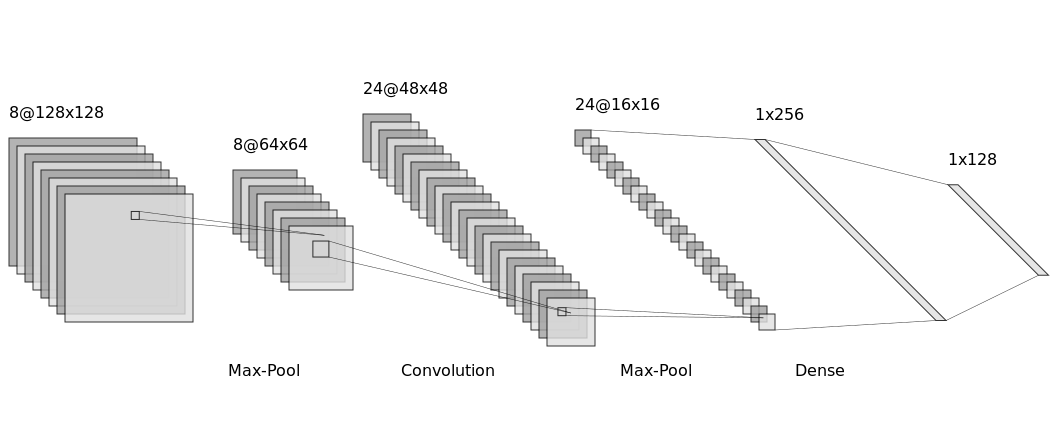
\includegraphics[scale=0.4]{images/redeconv.png}
    \caption{Exemplo rede neural convolucional.}
    \label{fig: cnn}
\end{figure}


As redes convolucionais, que seguem o modelo apresentado na figura \ref{fig: cnn}, geralmente recebem como entrada imagens e podem fazer extração de características e classificações a partir desses dados. Em casos de diagnóstico médico feito a partir da avaliação visual, como uma parte do diagnóstico da psoríase, por exemplo, o uso desses modelos seria adequado.

Uma alternativa à abordagem da \gls{cnn} é a arquitetura de \textit{Visual Transformers}. Essa arquitetura utiliza o algoritmo de \textit{Transformers} (figura \ref{fig:transformer-arch}) para análise de imagens, os \textit{transformers}, foram inicialmente propostos por \citeonline{Vaswani}. Diferente dos modelos recorrentes da época, que processavam informações de forma sequencial, o que impedia a paralelização eficiente dentro dos exemplos de treinamento em sequências longas e limitava o agrupamento de dados, o \textit{Transformer} abandona a recorrência. Em vez disso, ele se baseia inteiramente em um mecanismo de atenção para capturar dependências globais entre as entradas e saídas. 
Essa abordagem permitiu uma paralelização significativamente maior durante o treinamento e estabeleceu novos patamares de desempenho em tarefas como a tradução automática.

% Uma alternativa a abordagem da \gls{cnn} é a arquitetura de \textit{Visual Transformers}, essa arquitetura utiliza como base um algoritmo de atenção, a proposta inicial desse algoritmo tinha como objetivo propor uma solução aos modelos recorrentes da época para tarefas de tradução, esses outros modelos da época tinham uma natureza sequencial, o que impedia a paralelização dentro dos exemplos de treinamento \cite{Vaswani}. 

\begin{figure}
  \begin{minipage}[b]{0.6\textwidth}
    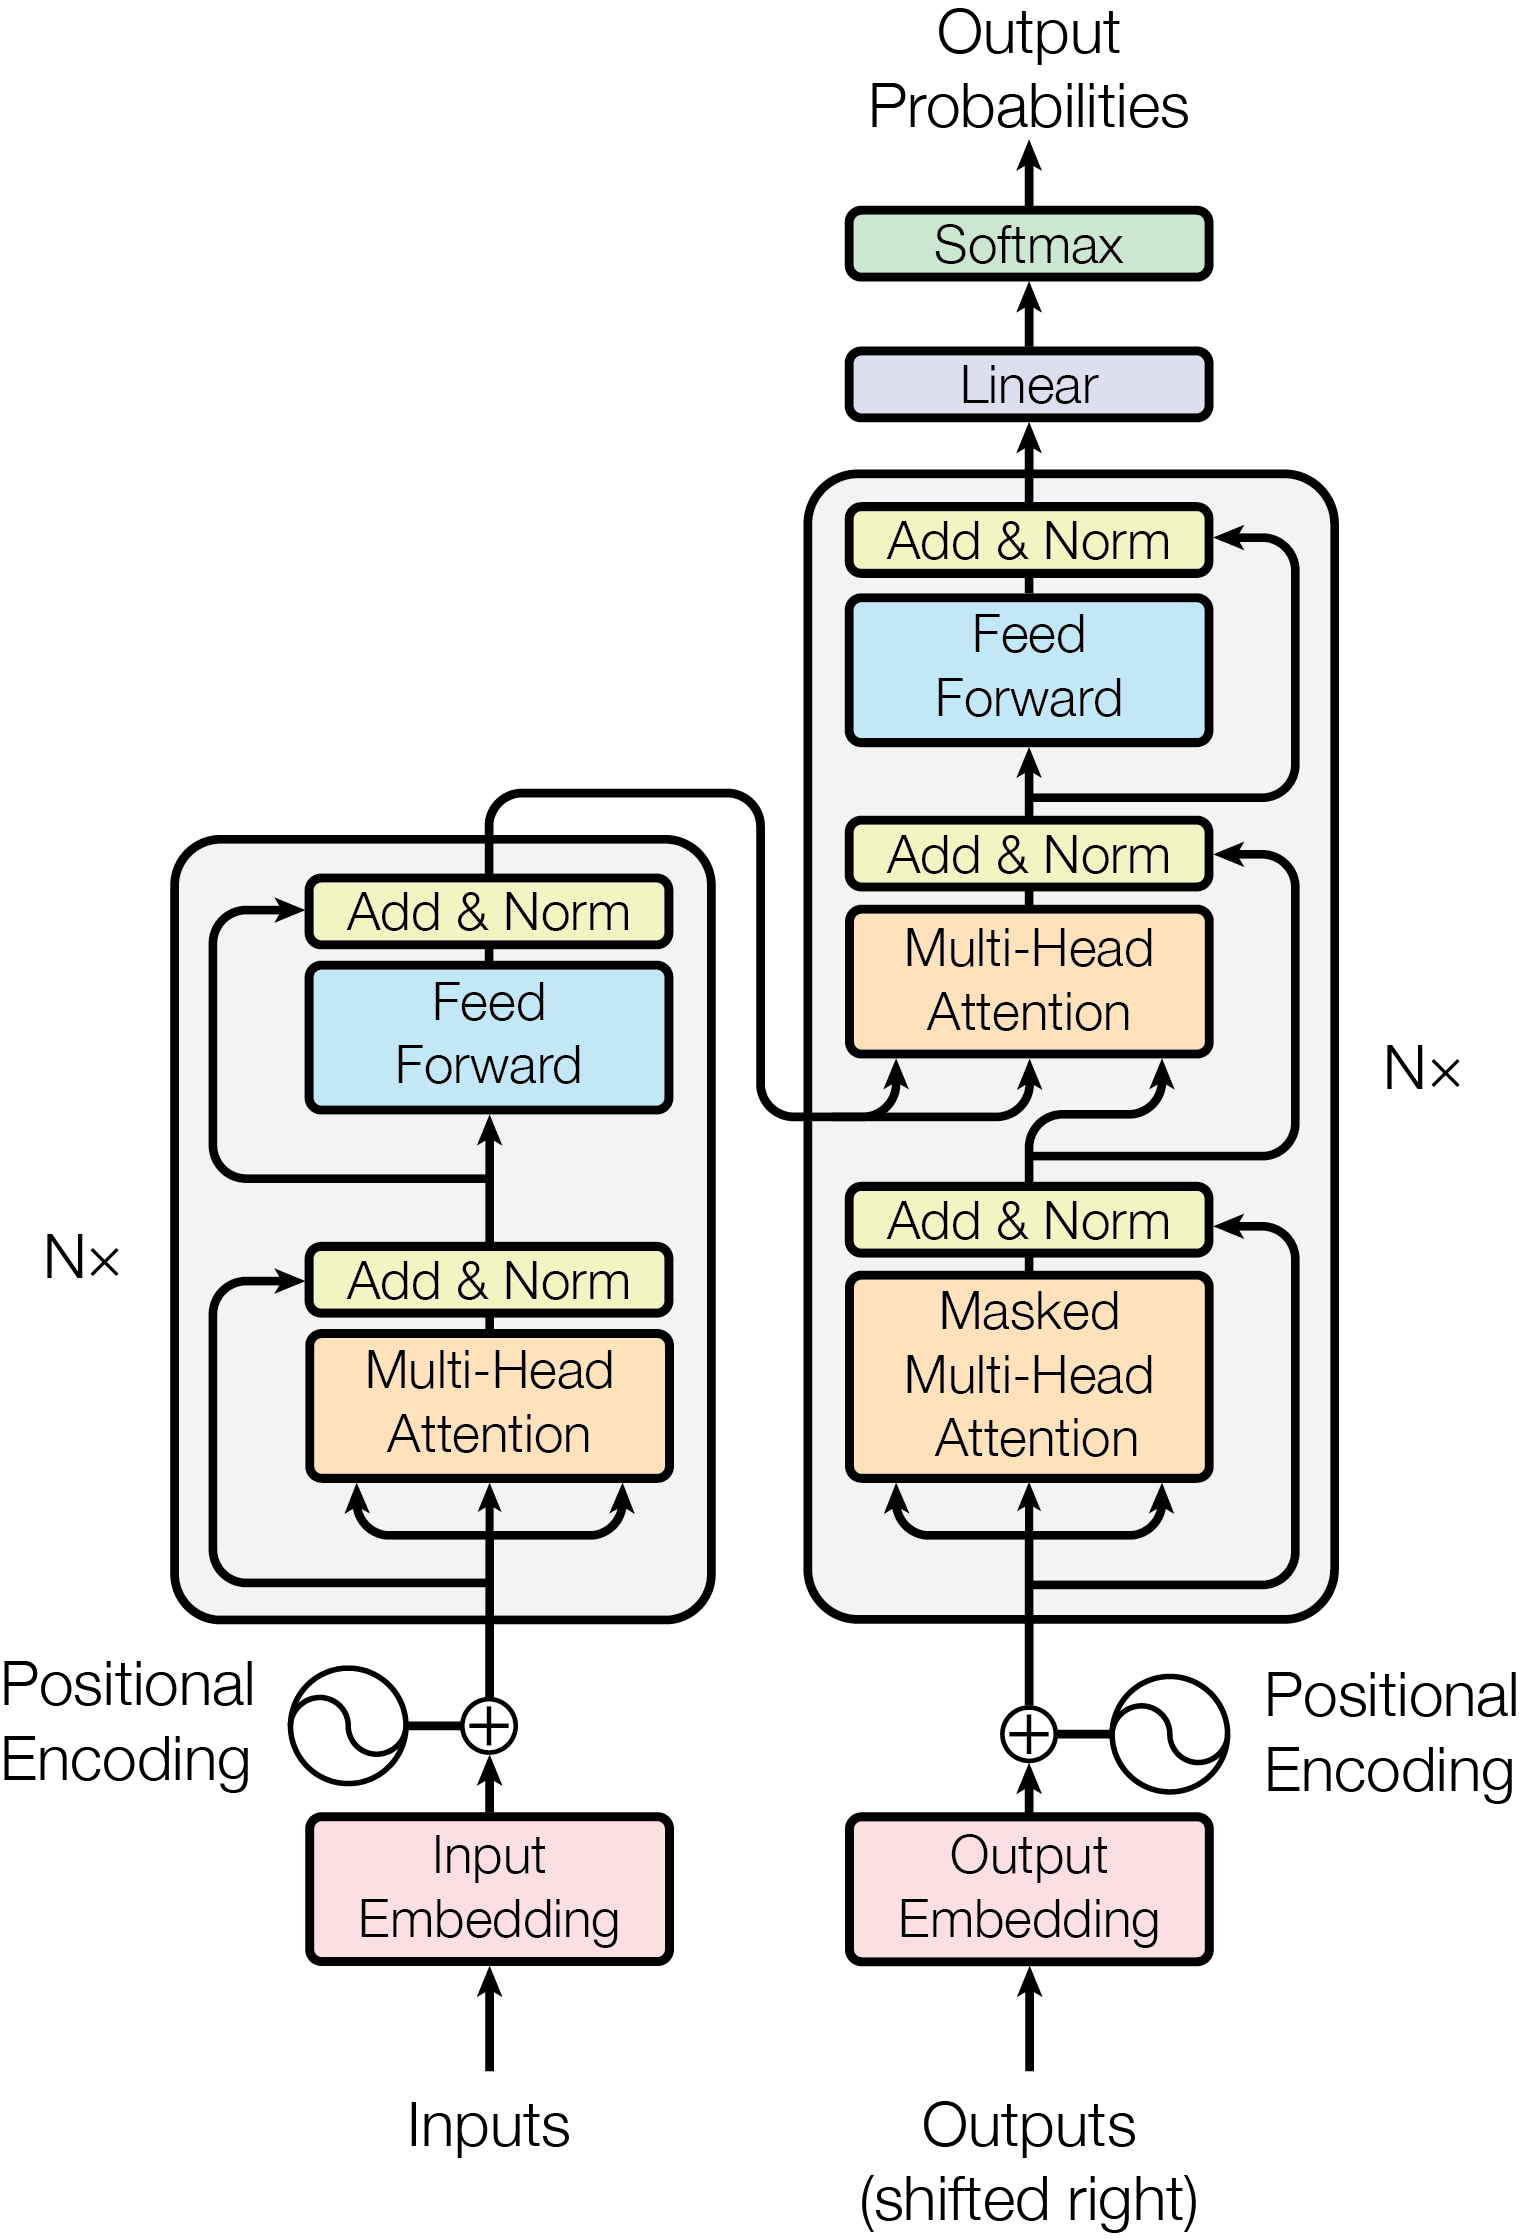
\includegraphics[scale=0.5]{images/ModalNet-21}
    \caption{Arquitetura do transformer. (\citeonline{Vaswani})}
    \label{fig:transformer-arch}
  \end{minipage}
  \begin{minipage}[b]{0.5\textwidth}
    \centering
    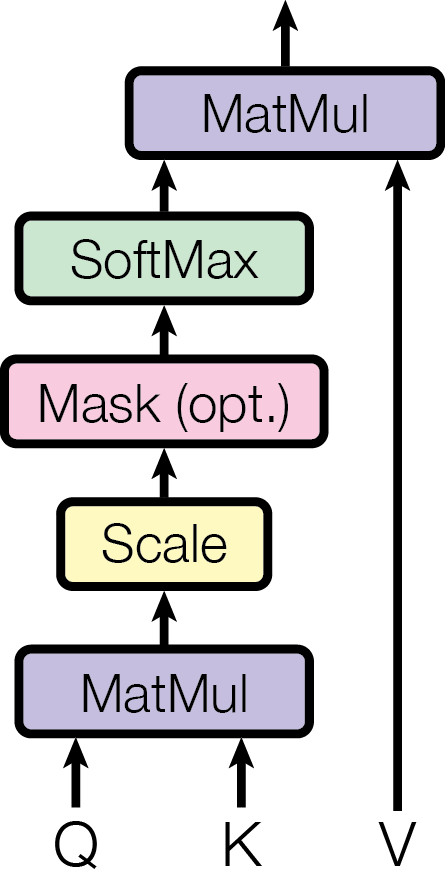
\includegraphics[scale=0.7]{images/ModalNet-19}
    \caption{Scaled Dot-Product Attention. (\citeonline{Vaswani})}
    \label{fig:dot-att}
  \end{minipage}
\end{figure}

\citeonline{Vaswani} define o mecanismo de autoatenção (\textit{self-attention}), demonstrado na figura \ref{fig:dot-att}, como um algoritmo que permite que o modelo pese a importância de diferentes partes da sequência de entrada ao gerar uma representação para cada elemento da sequência. As entradas são recebidas como vetores. Ao processar esse vetor, o modelo compara diretamente com todos os outros vetores na sequência de entrada simultaneamente em uma única camada, o que possibilita a paralelização, e determina quais são as mais relevantes para entender o contexto daquele elemento específico, diferentemente da \gls{cnn}, que consideram apenas as informações que se encontram no mesmo espaço do filtro definido, ou seja, contexto local. 
 Esse processo é realizado calculando scores de similaridade entre os elementos, permitindo que as dependências de longo alcance sejam capturadas de forma eficaz, sem as limitações sequenciais dos modelos recorrentes.

% \begin{figure}
%   \centering
%   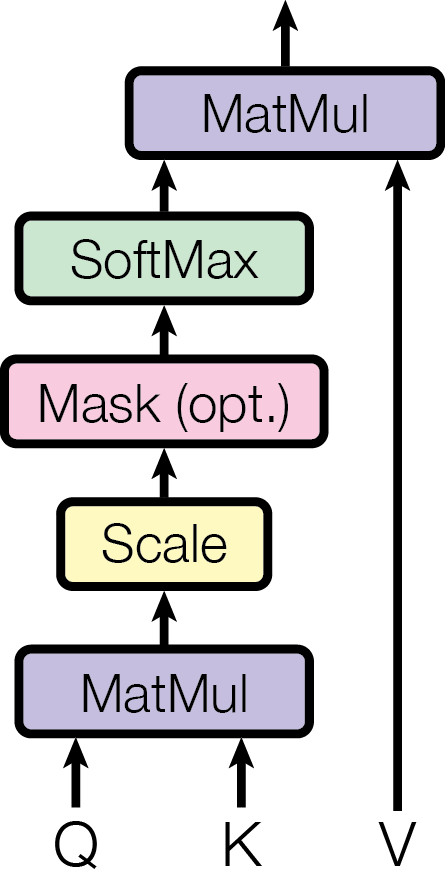
\includegraphics[scale=0.6]{images/ModalNet-19}
%   \caption{Scaled Dot-Product Attention.}
%   \label{fig:dot-att}
% \end{figure}
%
% Model overview. We split an image into fixed-size patches, linearly embed each of them, add position embeddings, and feed the resulting sequence of vectors to a standard Transformer encoder. In order to perform classification, we use the standard approach of adding an extra learnable classification token to the sequence. - peguei do artigo original
  
Os \textit{Visual Transformers} (figura \ref{fig:vit-arch}), por sua vez, dividem as imagens em patches de tamanhos fixos, diferentemente das \gls{cnn}s que processam pixels diretamente ou por meio de filtros convolucionais. Cada um desses patches é vetorizado e a esses vetores são adicionados embutimentos de posição (\textit{position embeddings}), para preservar a informação espacial original da imagem, após essa operação, essa sequencia passa por um \textit{encoder} padão que utiliza o algoritmo de atenção para aprender os padrões daquela sequência e as relações entre os diferentes patches da imagem. Para realizar tarefas de classificação, como a detecção de doenças de pele, um token de classificação extra, que é treinável, é adicionado à sequência, e sua saída final é usada para a previsão \cite{Dosovitskiy}.
\newline
\newline
\newline

% Imagem do artigo sobre visual transformers
\begin{figure}[h]
  \centering
    \begin{tabular}{c}
      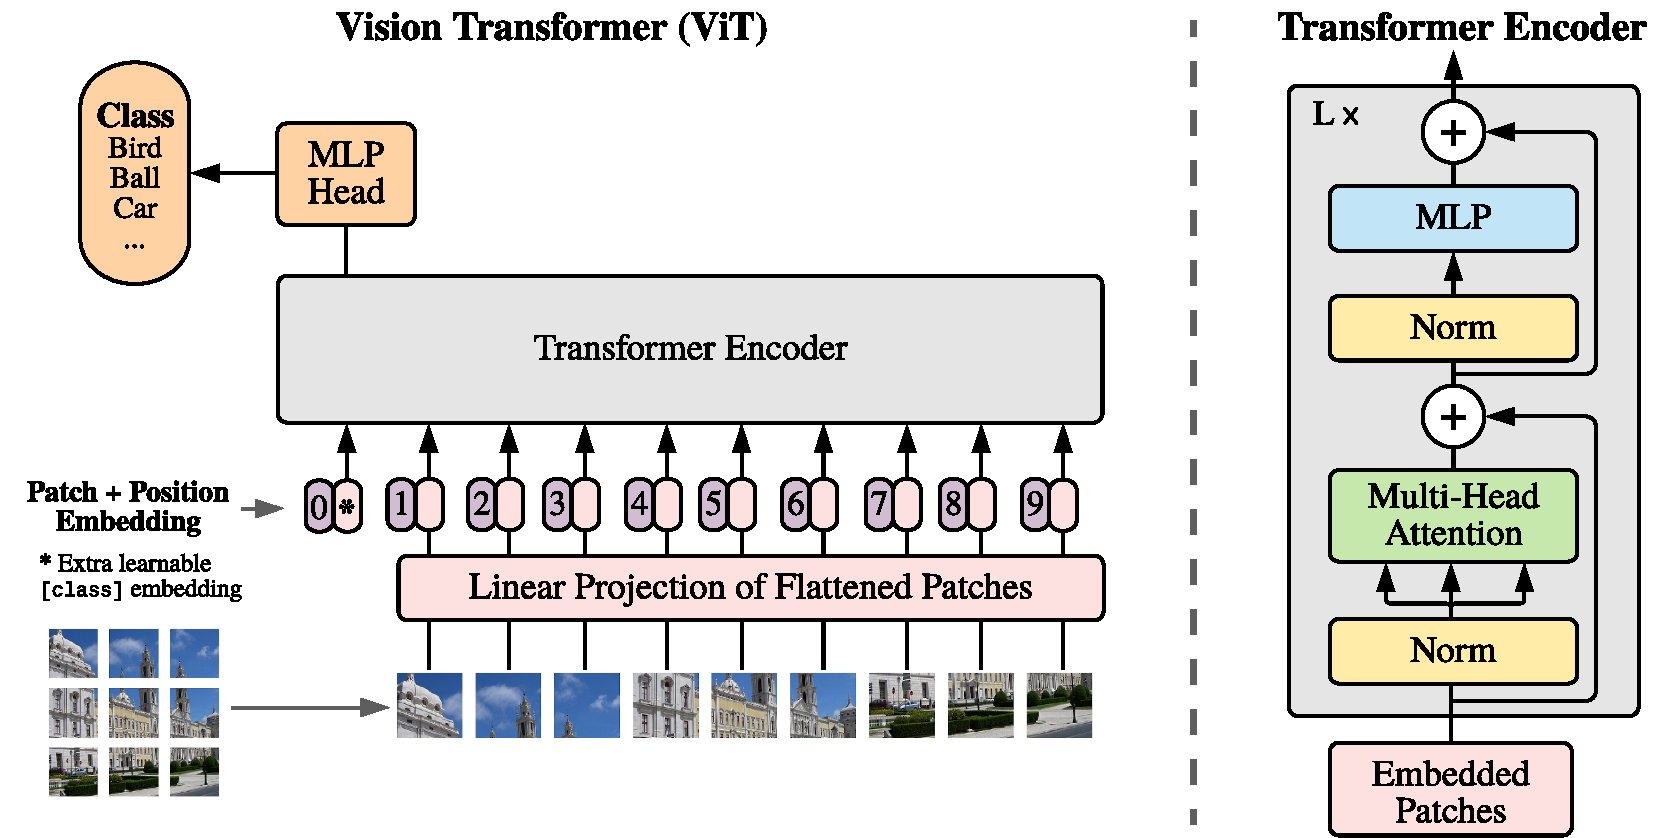
\includegraphics[scale=0.4]{images/model_scheme.pdf}
    \end{tabular}
    \caption{The Visual Transformer. (\citeonline{Dosovitskiy})}
    \label{fig:vit-arch}
\end{figure}

\subsection{Sobre Sistemas CAD}

Os primeiros estudos sobre análise quantitativa de imagens médicas por computador foram relatados na década de 1960. Porém, nos anos 80 surgiu uma nova abordagem, que assume que os sistemas CAD podem ser utilizados pelos profissionais da saúde como ferramenta e não para substituí-los. Assim, o objetivo principal desses sistemas é que a saída do CAD seja como uma “segunda opinião” para os médicos, para que estes façam a avaliação final. Nesse sentido, o uso dos sistemas CAD permite uma melhora na avaliação final em diferentes cenários, caso o médico esteja menos confiante sobre sua avaliação, a saída desse sistema tem a intenção de apoiar a avaliação final; e em uma situação onde o médico está mais confiante de sua avaliação, ele pode “descartar” a saída do computador. Alguns estudos afirmam que os sistemas CAD não precisam necessariamente se igualar ou superar a precisão na classificação em comparação aos profissionais na área da saúde, porém é importante ressaltar que quanto maior for o desempenho da máquina, melhor será o resultado final combinado \cite{DOI2007198}.

Para auxiliar na definição da metodologia do projeto de pesquisa, foi realizado um levantamento do estado da arte para as técnicas de classificação com imagens médicas. O processo de levantamento bibliográfico considerou o levantamento de artigos científicos nas bases científicas MDPI, IEEE, Elsevier e Scopus. Para realizar a busca dos artigos, foram utilizadas as palavras-chaves: “CAD”, “Computer Aided System”, “CAD convolution”, “psoriasis”, “CAD psoriasis”. Foram levantados 21 artigos considerando o filtro por título e resumo; dos quais, 13 foram detalhadamente analisados, com destaque para os trabalhos de Li (2020), Brinker (2019) e Doi (2007).

Li (2020), apresentou em sua pesquisa um sistema CAD para o diagnóstico de câncer de pâncreas. Nesse sistema, o autor utilizou um algoritmo baseado em support vector machine (SVM). Além desse algoritmo, o autor utilizou outras técnicas como o algoritmo LASSO, técnica de regularização usada principalmente para evitar o sobre ajuste do modelo e ajudar a selecionar as características importantes, e também propôs um modelo utilizando ensemble, que visa trazer mais robustez e melhorar a precisão do sistema através da construção e combinação de vários modelos. O algoritmo de ensemble usado para esse sistema foi o algoritmo bagging (bootstrap aggregating); nesse algoritmo várias subamostras são geradas aleatoriamente a partir do conjunto de dados original, com repetição e as previsões dos modelos individuais são combinadas para gerar uma previsão final. Esse sistema CAD atingiu uma precisão de 91.63\% para os dados na classe “Normal Stage - IV”, essa classe representa o estágio mais avançado da doença.

Já \citeonline{BRINKER201911}, apresentou em sua pesquisa um sistema CAD voltado para dermatologia, o modelo proposto superou dermatologistas na classificação de imagens de melanoma. Em seu trabalho, Brinker utilizou apenas imagens com uma qualidade avaliada como excelente, boa ou suficiente  pelos dermatologistas que participaram da pesquisa. O sistema CAD proposto foi desenvolvido usando uma arquitetura de redes neurais já conhecida, a ResNet50 e os dados vieram de fontes open-source (código aberto) e comprovados por biópsia. Considerando um intervalo de confiança (CI) de 95\%, após o treinamento do modelo, este atingiu uma sensibilidade de 82.3\% (95\% CI: 78.3–85.7\%) e especificidade de 77.9\% (95\% CI: 73.8–81.8\%), já os dermatologistas atingiram uma sensibilidade de 67.2\% (95\% CI: 62.6–71.1\%) e especificidade de 62.2\% (95\% CI: 57.6–66.9\%).


Ainda no contexto dermatológico, \citeauthor{DASH2020106240} apresenta um sistema CAD totalmente integrado, que é composto por três estágios: classificação, segmentação e avaliação da severidade da lesão. No primeiro estágio, o sistema é baseado numa arquitetura de redes convolucionais chamada de VGG-16, composta de 13 camadas convolucionais e 3 camadas totalmente conectadas. Neste trabalho, algumas alterações foram feitas nesse modelo, como a remoção de camadas “redundantes”, com o objetivo de reduzir a quantidade de parâmetros, tornando assim essa rede mais eficiente computacionalmente. A primeira parte do trabalho, que compõe a rede convolucional para classificação da doença, atingiu uma acurácia de 93.76\%.


Como já visto anteriormente, em sua grande maioria, esses sistemas são construídos para lidar com dados não estruturados, que é o caso de imagens. A visão humana, diferente dos computadores, é limitada à banda visual do \ac{EM}, já os aparelhos de processamento de imagens cobrem quase todo o espectro eletromagnético (EM), variando de ondas gama a ondas de rádio; basicamente esses dispositivos são capazes de trabalhar com imagens geradas por fontes que os seres humanos não estão acostumados a associar, entre esses tipos de fonte, estão: imagens geradas por ultrassons, microscopia eletrônica e imagens gerada por computador \cite{gonzalez2008digital}. 


Há uma grande vantagem na aplicação da visão computacional nesse setor, que por sua vez, estuda diferentes técnicas para trabalhar com imagens, como por exemplo, os já citados modelos de classificação, além de técnicas de extração de características, detecção de bordas, entre outras. Entre essas diversas técnicas, destacam-se os modelos baseados na arquitetura de redes neurais \cite{DOI2007198}.


Do mesmo modo que a visão computacional avança com suas técnicas na área da saúde, outra área que também se beneficia é o processamento digital de imagens, que possui uma relação muito forte com a visão computacional. Essa área de estudo está ligada principalmente com os conceitos de filtragem, transformações geométricas e restauração de imagens. O objetivo desses tratamentos nas imagens é prepará-las para análises posteriores, de modo a oferecer as técnicas necessárias para pré-processar e manipular imagens, antes de “alimentar” esses dados nas redes convolucionais \cite{gonzalez2008digital}.


